\documentclass{report}

\usepackage{float}
\usepackage{url}
\usepackage{graphicx}
\usepackage{listings}
\usepackage{color}
\usepackage{verbatim}
\usepackage[lined,linesnumbered,algochapter]{algorithm2e}
\usepackage{tikz}
\usetikzlibrary{arrows,automata}
\usepackage{xspace}
\usepackage{caption}
%\usepackage[colorlinks = true, urlcolor  = blue]{hyperref}
\usepackage{ucs}
\usepackage[utf8]{inputenc}

%\hypersetup{colorlinks=false, linkcolor=red}

\usepackage{ngerman}
\usepackage[ngerman, english]{babel}
\usepackage{bibgerm,cite}       % Deutsche Bezeichnungen, Automatisches Zusammenfassen von Literaturstellen
\usepackage[ngerman]{varioref}  % Querverweise

\DeclareCaptionFont{white}{\color{white}}
\DeclareCaptionFormat{listing}{\colorbox{gray}{\parbox{\textwidth}{#1#2#3}}}
\captionsetup[lstlisting]{format=listing,labelfont=white,textfont=white}

\lstset{language=Java,captionpos=b,tabsize=3,frame=lines,keywordstyle=\color{blue},commentstyle=\color{darkgreen},stringstyle=\color{red},numbers=left,numberstyle=\tiny,numbersep=5pt,breaklines=true,showstringspaces=false,basicstyle=\footnotesize,emph={label}}

\setcounter{secnumdepth}{2}
\setcounter{tocdepth}{3}

% another code presentation stlye
%\definecolor{dkgreen}{rgb}{0,0.6,0}
%\definecolor{gray}{rgb}{0.5,0.5,0.5}
%\definecolor{mauve}{rgb}{0.58,0,0.82}
%
%\lstset{frame=tb,
%  language=Java,
%  aboveskip=3mm,
%  belowskip=3mm,
%  showstringspaces=false,
%  columns=flexible,
%  basicstyle={\small\ttfamily},
%  numbers=none,
%  numberstyle=\tiny\color{gray},
%  keywordstyle=\color{blue},
%  commentstyle=\color{dkgreen},
%  stringstyle=\color{mauve},
%  breaklines=true,
%  breakatwhitespace=true
%  tabsize=3
%}

% define custom macros for specific formats or names
\newcommand{\uml}[1]{\texttt{#1}}
\newcommand{\cd}{\textsf{Class Diagram}}

\begin{document}
\pagestyle{plain}
\pagenumbering{roman}

\title{Risikomanagement}


\maketitle

\tableofcontents
\newpage

\pagenumbering{arabic}

% Kapitel
% --------------------------------------------------------------
\chapter{Definition und Grundlagen Risikomanagement}
\label{sect:grundlagen}


% --------------------------------------------------------------
\chapter{Software, Plattformen und Apps im Risikomanagement}
\label{sect:software}



% --------------------------------------------------------------
\chapter{Risikomanagement im Bereich Service und Data Clouds}
\label{sect:clouds}



% --------------------------------------------------------------
\chapter{Risikomanagnement im Kontext von Smart Technologien}
\label{sect:relevance}

\section{Neue IT-Risiken durch Smart Technologies (Internet of Things)}



Es ist nur mehr eine Frage der Zeit, bis alle „Dinge“ mit dem World Wide Web kommunizieren und Daten austauschen. Wie schön dies auch klingt und unser Leben dadurch auch in gewisser Weise erleichtert wird, verbergen sich hinter diesen Maßnahmen auch Risiken, die zum Teil auch neu sind. Diese Risiken bestehen sowohl für Unternehmen als auch für Verbraucher. Jedes Gerät, dass eine Internetverbindung hat, ist zugleich eine offene Tür für Angreifer. Einige dieser Geräte haben Betriebssysteme wie Linux oder Android installiert und bringen auch dieselben Stärken und Lücken mit.
Überwachung spielt hier eine sehr wichtige Rolle. Wenn zu bestimmten Zeitpunkten auffällige Geschehnisse auftreten, könnte dies ein Indiz dafür sein, dass etwas nicht stimmt. Mit einer Überwachungssoftware würde dieser Prozess einfach gestoppt werden. 
\\
\\
Durch die gute Vernetzung der intelligenten Technologien, kann sobald sich ein Virus in ein Gerät eingenistet hat, sich ganz einfach auf andere Geräte verbreiten. Im Falle der Datenspionage kann die Privatsphäre noch stärker verletzt werden. Da die Geräte vernetzt sind und jedes davon verschiedene User Informationen enthalten, ist es für den Angreifer noch leichter alle Daten auf einen Schlag zu bekommen.
\\
\\
Wenn wir die Gruppe Wearables betrachten gibt es Geräte die wichtige Funktionen Im menschlichen Körper steuern und dadurch unterstützen. Dies bringt ein Lebensgefährliches Risiko mit. Sei es ferngesteuerte Insulinpumpen oder Geräte für die Stimulation des Herzens. Hier dürfen keine Sicherheitslücken existieren, da ansonsten die Personen die diese Wearables tragen und benützen, in Lebensgefahr gebracht werden.
\\
\\
Unternehmen, die den Smart Technology Trend mit dem sogenannten „Bring your own Device“ – Betriebsvereinbarungen verfolgen, gehen ebenfalls ein hohes Sicherheitsrisiko ein. Private Geräte können nur teilweise überwacht und kontrolliert werden, wodurch sensible Unternehmensdaten in falsche Hände geraten können. Um einen sinnvollen Einsatz der Smart Technologies im Unternehmen zu gewährleisten, müssen diese auch immer online sein, da ansonsten mit Ausfällen ein Schaden angerichtet werden könnte.
\\
\\
\begin{figure}[hbtp]
\centering
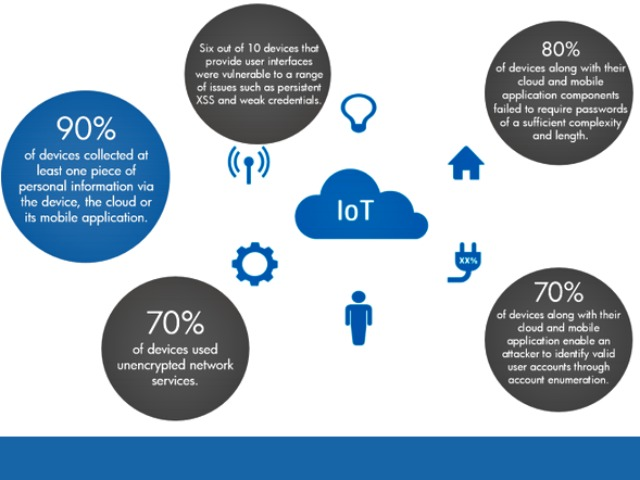
\includegraphics[scale=0.5]{hp-iot-security.jpg}
\caption{HP Studie Internet of Things (http://www8.hp.com/h20195/V2/GetPDF.aspx/4AA5-4759ENW.pdf)}
\end{figure}

\section{Spezifische Bereichsrisiken}

\subsection{Smart Home}

\textbf{Elektronik:} Intelligente Haushaltsgeräte sowie Beleuchtungen und Fenster schaffen zusätzliche Belastung in der Hauselektronik. Smarte Technologien die über Web-basierende Apps angesteuert werden, sind anfällig für Überspannungen und Blitzschlag. Diese haben konsequenterweise Einfluss auf das gesamte elektrische System im Haus. Das Motherboard des Steuergerätes der Smart Home Technologie könnte dadurch auch einen Schaden bekommen. Hohe Reparaturkosten wären dann die Folgen.
\\
\\
\textbf{Web Sicherheit:} Die Verwendung moderner und innovativer Technologie Zuhause, erleichtert uns das Leben und kann auch viel Geld einsparen. Eine Waschmaschine die mit dem WLAN verbunden ist und den Waschgang erst dann startet wenn der Strompreis am günstigsten ist, würde im Haushalt einiges an Geld einsparen. Jedoch jedes Gerät, das mit dem Internet verbunden wird, wird Möglicherweise auch zugänglich für andere. 
Da diese Systeme zurzeit von kleineren Unternehmen entwickelt werden, kann die Sicherheit schwach ausfallen.
\\
\\
\textbf{Privatsphäre:} Nachdem ein Smart Home System gehackt wurde, besteht natürlich auch das Risiko, dass die Privatsphäre verletzt werden kann. Es kann Zugang zu den Kameras, zum Smart TV oder Babyfon verschafft werden. In den USA gab es einen Vorfall, wo ein Hacker das Kind durch das Babyfon beschimpft hat.\footnote{http://www.n24.de/n24/Wissen/Technik/d/3379940/-wach-auf--du-kleine-schlampe-.html}
Gewohnheiten sowie Urlaubsaufenthalte können ausgeforscht werden, was dazu führt, dass Kriminelle auch physischen Schaden anrichten können.
\\
\\
\textbf{Versicherungsdeckung:} Wenn Smart Home Technologies verwendet werden, muss auch über eine Fern Überwachung gedacht werden. Dies dient nicht nur zur persönlichen Sicherheit sondern auch für die Versicherungsdeckung. Es müssen über Firewalls und Passwortschutz nachgedacht werden.

\subsection{Smart Factory (Industrie 4.0)}

So groß die Risiken sind so groß sind auch die Vorteile. Maschinen und Bauteile können sich verständigen, dadurch kann extrem genau in der Produktion kalkuliert werden. Das bringt Ressourceneffizienz weniger Materialeinsatz und eine bessere Ökobilanz. 
Durch die Vernetzung der Einheiten in der Produktion, sind kleinere Subsysteme immer enger gekoppelt und voneinander Abhängig. Dadurch steigt die Komplexität und parallel auch das Risiko.
\\
\\
Während der Einsatz von intelligenter Industrie den menschlichen Fehler als Risikofaktor senkt, könnten bei Problemen mit den Maschinen menschlicher Einsatz benötigt werden. Diese Personen müssen bestimmte Qualifikationen und Fertigkeiten besitzen um derartige Probleme lösen zu können. In so einem Fall kann möglicherweise die ganze Produktionskette lahmgelegt werden. Der "menschliche Faktor" geht sozusagen verloren. Zum Beispiel: Was passiert wenn eine Gasleitung undicht wird und es ist keiner da der es bemerkt. Solche Risiken müssen aufgespürt werden und in den Designprozess mit einfließen.
\\
\\
Das finanzielle Risiko spielt demnach auch eine wesentliche Rolle. Wenn neue intelligente Technologien in der Industrie eingesetzt werden, stellt sich die Frage ob es die Mitarbeiter dazu gibt, die diese Geräte zu bedienen wissen. Es werden eventuell neue Leute mit neuen Fertigkeiten benötigt die mehr Kosten. Was passiert wenn die Integration der intelligenten Maschinen in den Arbeitsablauf fehlschlägt. Das Unternehmen könnte die geforderte Produktionsmenge nicht mehr einhalten. Dies könnte im weiteren zu einer Rufschädigung führen, was für ein Unternehmen das schlimmste wäre.
\\
\\
Die bisher besprochenen Fälle können bei gut durchdachtem Risikomanagement kalkuliert und bewältigt werden. Was ist jedoch wenn ein Hacker oder ein Mitarbeiter die intelligenten Maschinen mit einem Virus infiziert. Dies würde alle schlimmen Szenarien ermöglichen. Herunterfahren von Maschinen, Produktionsdefekte, Umweltschäden bis hin zur Wirtschaftsspionage wichtiger Prozesse und Daten. Der Erholungsprozess eines Unternehmens von solch einer Attacke könnte über Jahre hinweg andauern.

Versicherbarkeit?
Hohe Wartungskosten

\subsection{Smart Car}

Autos werden immer intelligenter. Selbstparksysteme und Abstandsregeltempomaten sind bereits auf dem Markt. Autos kommunizieren mit anderen Autos und kontrollieren das Fahrzeug für mehr Sicherheit und Bequemlichkeit. Diese neuen intelligenten Technologien kommen bald in die Massenproduktion und werden unvermeidlich. Wie auch in den anderen Bereichen, bietet diese Innovation reichlich Platz an Risiken.
Im Jänner 2015 wurde im System „ConnectedDrive“ von BMW eine Sicherheitslücke entdeckt. Diese Lücke erlaubte die Autos mit dem Mobiltelefon per GSM-Funk zu öffnen. Der Grund dafür war die unverschlüsselte Kommunikation, welche BMW aber abstreitet. Es waren 2,2 Millionen Autos davon betroffen und der Fehler existierte über Jahre inweg. inweg\footnote{http://www.spiegel.de/auto/aktuell/adac-entdeckt-it-sicherheitsluecke-bei-bmw-connected-drive-a-1015819.html}
\\
\\
Assistenzsysteme, die für Bremsen und halten der Spur zuständig sind, können von außen manipuliert werden. Diese Manipulation hat zur Folge, dass falsche Signale simuliert werden und so die Kontrolle des Autos in andere Hände übergehen kann. Je stärker die Kopplung der Systeme zueinander steht, desto leichter ist es für Eindringlinge das System zu überlisten.
\\
\\
Mit der Einführung des Smart Cars muss die Gesellschaft auch lernen umzudenken. Die Sicherheit, Unfälle durch menschlichen Fehler zu vermeiden steigt enorm, jedoch müssen Fahrzeuge nun vor Hackangriffen geschützt werden. Im Falle eines Unfalles, der durch einen Hackangriff verursacht wurde, stellt sich die Frage, wer die Schuld trägt? Diese und weitere Fragen müssen sorgfältig behandelt und geklärt werden.
\\
\\
Der Umgang mit persönlichen Daten spielt auch eine sehr wichtige Rolle. Autos speichern und übertragen viele persönliche Daten wie Bewegungsprofile, Fahrweise, Verbrauch, Telefonbücher und sogar Kreditkartendaten bei automatisierter Bezahlung von Parkgebühren. Diese Daten sind für Cyberkriminelle von hohem Wert.
\\
\\
Da bei Smart Cars zwei unterschiedliche Branchen aufeinandertreffen, bringt dies auch ein gewisses Risiko mit.  Während in der IT monatliche Zyklen Standard sind, ist man in der Autoindustrie eher den Jahreszyklus gewöhnt. 

\section{Best Practices beim Management von Smart-Technology-Risiken}

Eine routinierte Sicherheitsüberprüfung auf den Geräten und den verbundenen Komponenten ist das A und O. Aufgrund der Menge der Geräte muss diese automatisiert erfolgen. Die zu überprüfenden Komponenten sind:

\begin{itemize}
\item Web-Schnittstelle
\item Netzwerkübertragung
\item Ports
\item Authentifizierung / Autorisierung
\item Cloud communication
\end{itemize}
Es müssen Securiy-Policies entwickelt werden die jedes einzelne Gerät erfüllen muss. Wenn diese Standards einmal aufgesetzt und danach aktuell gehalten werden, ist das eine hohe Risikominimierung.
\\
\\
Damit die Sicherheit auch Gewährleistet ist, muss dieser Aspekt im ganzen Product-Lifecycle angewandt werden. Die frühe Begutachtung von Prozessergebnissen hält das Risiko gering. Softwareupdates sind somit bei Auftreten von Fehlern sehr wichtig. Wenn diese Updates schnell und routiniert eingespielt werden, bleibt das System bzw. die Geräte immer auf dem neuesten Sicherheitsstand.


\bibliographystyle{acm}
\bibliography{risk2015}

\end{document}
